\chapter{Implementationsdetails}
\label{chap:implementierung}
In diesem Kapitel werden die Funktionalitäten der Pipeline zusammengetragen. Um die Anforderungen genauer zu beschreiben, wird ein Use-Case-Diagramm und ein Flussdiagramm dargestellt und beschrieben. Zudem werden konkrete funktionale und nichtfunktionale Anforderungen des Systems erfasst. Abschließend werden verwendete Technologien und Implementationsaspekte genauer beschrieben.
\section{Beschreibung des entwickelten Systems}
\label{sec:beschreibungsystem}
\todo{danach wie muss ich software zusammenwürfeln um das was ich aktuell an infos habe zu template umformulieren.}\\
Es wird eine Lösung gesucht, die eine effiziente Verarbeitung von \emph{Bedarfsmeldungen} durchführen kann. Welche Aspekte in einer Bedarfsmeldung relevant sind, wurde bereits im Kapitel \ref{chap:erwartungshaltung} näher erläutert. Auf Basis welcher Methodiken und Ansätze die relevanten Informationen extrahiert werden können, wurde in Kapitel \ref{sec:literaturueberblick} dargestellt. Nun gilt es eine Lösung zu entwickeln, die diese Ansätze in einem System implementiert und Möglichkeiten zur Evaluation bietet. Die Idee ist es, eine Pipeline zu entwickeln, die Möglichkeiten zum laden von \emph{Bedarfsmeldungen} bietet. Damit alle Ansätze und Methoden zur Extraktion von Informationen gut funktionieren und vergleichbar bleiben, wird eine Übersetzungsfunktion der \emph{Bedarfsmeldungen} benötigt. Auch wenn die \emph{Bedarfsmeldungen} in den meisten Fällen auf Deutsch sind, hilf es diese zu übersetzen, damit keine Unterschiede in der Ergebnisqualität resultiert, da einige Methoden und Ansätze auf Basis von Englischen Trainingssätzen trainiert wurden. Schließlich müssen alle aus Kapitel \ref{sec:literaturueberblick} untersuchten Ansätze implementiert und nutzbar sein. Sie sollen die Möglichkeit haben \emph{Bedarfsmeldungen} als Input zu erhalten und eine Ausgabe zurückzugeben. Zur besseren Evaluationsmöglichkeit soll das System modular sein, damit Methoden und Ansätze nach belieben durchgetauscht werden können. Zur Überprüfung der Laufzeit soll eine Zeitmessung verfügbar sein, die die Zeit zwischen dem Start und der Beendigung des Systems zurückgibt.\\

\todo{erzählen was die Pipeline leisten soll, im Falle vom Hybrid wird wahrscheinlich noch data-fusion gebraucht, vektorisierung eventuell auch noch für cosine similarity}
\newpage
\section{Use-Case}
\label{sec:usecase}
In diesem Kapitel werden die Interaktionen zwischen Benutzer und System beschrieben. Dazu wird ein Use-Case-Diagramm angefertigt, das eine grafische Übersicht über alle Anwendungsfälle bietet.
\begin{figure}[H]
	\centering  
	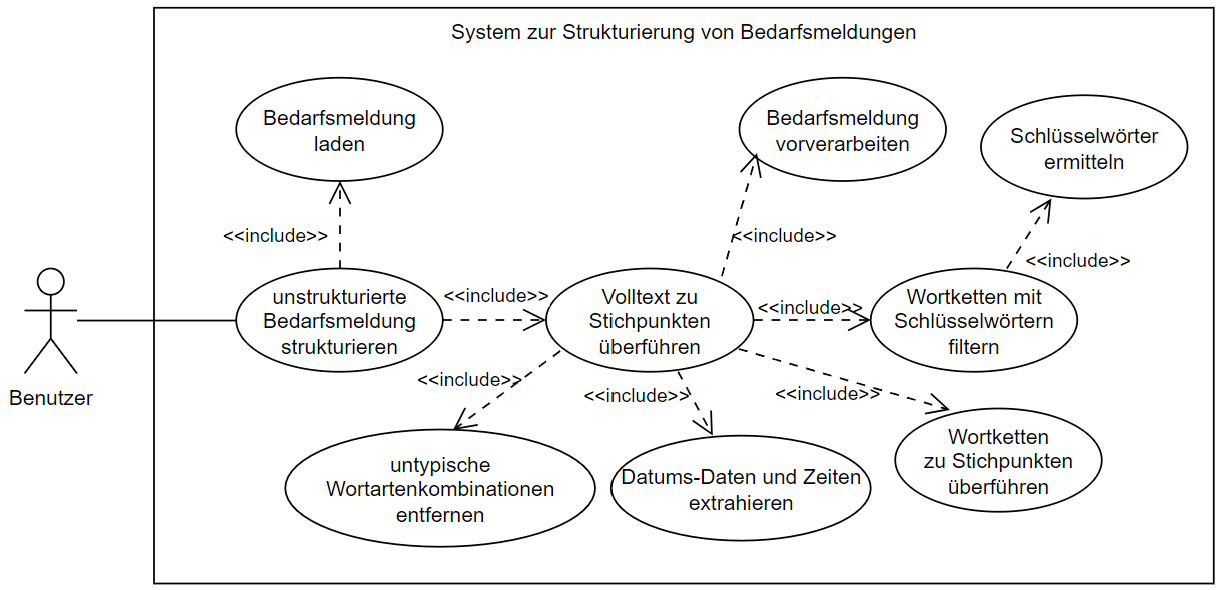
\includegraphics[width=\linewidth]{Abbildungen/use-case.png}
	\caption{Use-Case Diagramm der Pipeline.}
	\label{fig:usecasediagrammwirklich}
\end{figure}\mbox{} \\
In der Abbildung \ref{fig:usecasediagrammwirklich} ist das Use-Case Diagramm zur Pipeline. Es existiert ein Akteur. Dieser hat die Möglichkeit eine oder mehrere \emph{Bedarfsmeldungen} zu laden. Zudem kann diese ins Englische übersetzt werden. Darüber hinaus kann die \emph{Bedarfsmeldung} durch \emph{Preprocessing} vorverarbeitet werden und irrelevante Wörter und Zeichen aus der \emph{Bedarfsmeldung} ausschließen. Der Benutzer kann die Methoden \emph{TF-IDF}, \emph{TextRank}, \emph{N-Gram}, \emph{POS-Tagging} und \emph{NER} mit der \emph{Bedarfsmeldung} anwenden. Wenn mehrere Methoden in der Pipeline sind, können die Resultate durch die Anwendung von \emph{Data-Fusion} zusammengeführt werden.
\section{Anforderungen}
Im Folgenden werden die funktionalen sowie nichtfunktionalen Anforderungen des Systems beschrieben. Diese Informationen wurden aus der Beschreibung des Systems aus Kapitel \ref{sec:beschreibungsystem} und dem Use-Case aus Kapitel \ref{sec:usecase} hergeleitet und bilden den Rahmen des Systems.
\subsection{Funktionale Anforderungen}
Die funktionalen Anforderungen beschreiben konkrete Funktionalitäten des Systems. Dazu werden zusammengehörende Anforderungen nummeriert und im Falle der Systemanforderungen in detaillierte Unterpunkte aufgelistet und beschrieben.
\paragraph{Benutzeranforderungen}
\begin{enumerate}
	\item Dem Benutzer soll es möglich sein, Extraktionsmethoden austauschen zu können.
	\item Dem Benutzer soll es möglich sein, die Laufzeit des Systems zu sehen.
\end{enumerate}
\todo{vielleicht dann auch die evaluationsschritte einbauen}
\paragraph{Systemanforderungen}
\begin{enumerate}[label=1.\arabic*]
	\item Die \emph{Bedarfsmeldungen} sollen geladen werden können.
	\item Beim laden können eine oder mehrere \emph{Bedarfsmeldungen} geladen werden.
	\item Das System soll die Datenformate \emph{.txt} und \emph{.json} unterstützen.
\end{enumerate}
\begin{enumerate}[label=2.\arabic*]
	\item Die Bedarfsmeldungen sollen ins Englische übersetzt werden können.
\end{enumerate}
\begin{enumerate}[label=3.\arabic*]
	\item Das System soll Methoden des Preprocessing zur Bereinigung eines Volltextes implementiert haben.
	\item Das Preprocessing soll ein Volltext als Eingabe erhalten.
	\item Das Preprocessing soll den Volltext als Ausgabe zurückgeben.
\end{enumerate}
\begin{enumerate}[label=4.\arabic*]
	\item Das System soll die Methode \emph{TF-IDF} als Modul implementiert haben.
	\item Das Modul soll die Möglichkeit haben ein Volltextes als Eingabe für die implementierte Methode mitzugeben.
\end{enumerate}
\begin{enumerate}[label=5.\arabic*]
	\item Das System soll die Methode \emph{TextRank} als Modul implementiert haben.
	\item Das Modul soll die Möglichkeit haben ein Volltextes als Eingabe für die implementierte Methode mitzugeben.
\end{enumerate}
\begin{enumerate}[label=6.\arabic*]
	\item Das System soll die Methode \emph{N-Gram} als Modul implementiert haben.
	\item Das Modul soll die Möglichkeit haben ein Volltextes als Eingabe für die implementierte Methode mitzugeben.
\end{enumerate}
\begin{enumerate}[label=7.\arabic*]
	\item Das System soll die Methode \emph{POS-Tagging} als Modul implementiert haben.
	\item Das Modul soll die Möglichkeit haben ein Volltextes als Eingabe für die implementierte Methode mitzugeben.
\end{enumerate}
\begin{enumerate}[label=8.\arabic*]
	\item Das System soll die Methode \emph{NER} als Modul implementiert haben.
	\item Das Modul soll die Möglichkeit haben ein Volltextes als Eingabe für die implementierte Methode mitzugeben.
\end{enumerate}
\begin{enumerate}[label=8.\arabic*]
	\item Das System soll die Möglichkeit haben die Laufzeit des Systems zu messen.
	\item Der Startzeitpunkt wird beim Systemstart festgehalten.
	\item Der Endzeitpunkt wird beim Systemstop festgehalten.
	\item Die Differenz aus dem Start- und Stop- Zeitpunkt wird ermittelt.
\end{enumerate}
\subsection{Nichtfunktionale Anforderungen}
Hierbei handelt es sich um qualitätsbezogene Anforderungen. Diese umfassen nicht konkrete Funktionen des Systems, sondern stellen Rahmenbedingungen des Systems im Ganzen zusammen.
\begin{enumerate}
	\item Das System soll modular aufgebaut sein, um die Extraktionsmethoden austauschen zu können.
	\item Das System soll in der Lage sein, mehrere \emph{Bedarfsmeldungen} laden zu können.
\end{enumerate}
\newpage
\section{Systemablauf}
\todo{Flussdiagramm beschreiben und in der Einleitung nicht vergessen im Ablauf anzupassen dass das kein Klassendiagramm mehr ist}
\begin{figure}[H]
	\centering  
	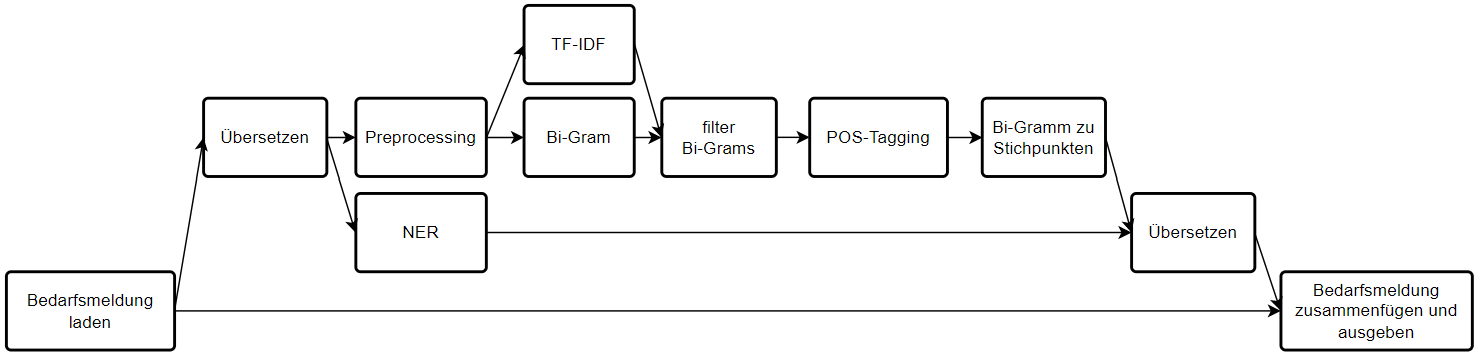
\includegraphics[width=\linewidth]{Abbildungen/flowchart.png}
	\caption{Flussdiagramm der Pipeline.}
	\label{fig:flowchart}
\end{figure}\mbox{} \\
\section{Details zur Implementierung der Pipeline}
Dieses Kapitel beschreibt den technischen Entwicklungsprozess zur Umsetzung der Anforderungen des Systems. Die Implementierung fokussiert sich auf die Umsetzungen von Technologien und Funktionsweisen verschiedener Anforderungen. Zudem wird die Struktur des Projektes aufgezeigt.
\subsection{Umsetzung}
Die Pipeline wurde in der Programmiersprache Python umgesetzt. Python hat sich zu einer der populärsten interpretierten Programmiersprachen entwickelt \cite{mckinney2012python}. Die Programmiersprache eignet sich insbesondere für die Erstellung kleiner Programme und Skripte, die zur Automatisierung von Aufgaben eingesetzt werden können \cite{mckinney2012python}. Python hat eine große und aktive Community für wissenschaftliche Berechnungen und Datenanalysen hervorgebracht und hat sich in den letzten Jahren zu einer der wichtigsten Sprachen für Data Science, maschinelles Lernen und allgemeine Softwareentwicklung in Wissenschaft und Industrie entwickelt \cite{mckinney2012python}. Python unterstützt Modularität, wodurch ein Teil der Anforderungen somit abgedeckt werden kann. Das Ziel der Arbeit besteht nicht in der Erweiterung der Verfahren, sondern in der Evaluierung ihrer Eignung zur Extraktion relevanter Informationen aus \emph{Bedarfsmeldungen}. Dadurch erfolgt die Implementierung der Methoden aus den Anforderungen nicht manuell, sondern es wurde auf bereits existierende Bibliotheken zurückgegriffen.
\subsection{Projektstruktur}
\label{sec:projektstruktur}
Das Projekt wird in einem git Repository gespeichert und versioniert. Die Projektstruktur ist ohne zusätzliche Konfigurationsdateien wie folgt aufgebaut:
\dirtree{%
	.1 .git/.
	.2 modules/.
	.3 ner.py.
	.3 nGram.py.
	.3 preprocessing.py.
	.3 readRequirements.py.
	.3 textRankingAlgorithm.py.
	.3 tfIdf.py.
	.3 transformRequirements.py.
	.3 translate.py.
	.2 requirements/.
	.3 jiraTickets.json.
	.3 ....
	.2 app.py.
	.2 ....
}
Die einzelnen Module aus dem Flussdiagramm in Kapitel \ref{fig:flowchart} sind im Verzeichnis \url{modules/} in separaten \url{.py} Dateien gelagert. Die \emph{Bedarfsmeldungen} werdem im \url{requirements/}-Verzeichnis gespeichert. Diese können die Endung \url{.txt} bei einzelnen und \url{.json} bei mehreren \emph{Bedarfsmeldungen} haben. Die Datei \url{app.py} ist der Kern der Pipeline. Diese importiert alle Module und kann über den Befehl \lstinline{> py app.py}
 das System starten.
\subsection{Modulimplementationen}
Nachfolgend werden Implementationsdetails zu den einzelnen Modulen gegeben. Dabei werden verwendete Bibliotheken und Code-Details näher erläutert.
\paragraph{Dateiformat}\mbox{}\\
Die \emph{Bedarfsmeldungen} wurden über die Jira-Schnittstelle extrahiert und im Verzeichnis \url{requirements/jiraTickets.json} gespeichert. Zur Eingrenzung der Datenmenge wurde ein Filter angewendet, der nur die \emph{offenen} und \emph{eskalierten} \emph{Bedarfsmeldungen} zurückgibt. Diese sind die relevanten und noch aktuellen \emph{Bedarfsmeldungen}. Zudem wurden alle unrelevanten Felder herausgenommen. Die Daten aus der Jira-API bestehen namentlich aus \emph{customfields} mit einer angehangenen ID. Der Softwareprototyp formt die unstrukturierten Fields in \emph{Bedarfsmeldungs}-Objekte um.
\begin{center}
	\begin{tabularx}{1\textwidth} { 
			| >{\raggedright\arraybackslash}X 
			| >{\raggedright\arraybackslash}X
			| >{\raggedright\arraybackslash}X | }
		\hline
		Display-Felder & Jira-API-Felder & Objekt-Felder \\
		\hline
		\hline
		Überschrift & summary & header\\
		\hline
		Rolle & customfield\_15321 & role\\
		\hline
		Aufgaben & customfield\_10288 & tasks\\
		\hline
		Skills & customfield\_10296 & skills\\
		\hline
		Skill-Level & customfield\_15322 & skillLevel\\
		\hline
		Kunde & customfield\_10279 & customer\\
		\hline
		Einsatzort & customfield\_10297 & location\\
		\hline
		Beginn & customfield\_10293 & timePeriod\\
		\hline
		Ende & customfield\_10294 & timePeriod\\
		\hline
		Tagessatz & customfield\_10298 & dailyRate\\
		\hline
	\end{tabularx}\\
	\captionof{table}{Übersicht der Datenfelder}
	\label{tab:jiradaten}
\end{center}
In der Tabelle \ref{tab:jiradaten} ist in der ersten Spalte eine Übersicht der Datenfelder, wie diese in der Abbildung \ref{fig:jiraafter} mit dem Mockup einer standardisierten \emph{Bedarfsmeldung} auftauchen. In der zweiten Spalte sind die dazugehörigen Feldernamen, die in der \url{jiraTickets.json} enthalten sind. Die dritte Spalte spiegelt die jeweiligen Namen innherhalb des Bedarfsmeldungs-Objekts im Prototypen wieder. Das Bedarfsmeldungs-Objekt dient der strukturierte Handhabung innerhalb des Systems.

%Um einen Freitext aus einer einzelnen \emph{Bedarfsmeldung} für die Pipeline zu laden werden Daten mit der Endung \url{.txt} verwendet.
%\begin{lstlisting}[caption={Implementation der Methode read() des Moduls \emph{readRequirements.py}}, label=lst:read]
%	def read(filename):
%		path = os.path.join(PATH, filename)
%		file = open(path, "r", encoding="utf-8")
%		content = file.read()
%		file.close()
%		return content
%\end{lstlisting}
%Im Listing \ref{lst:read} ist die Implementierung der Methode zum laden eines Freitextes dargestellt. Durch ein mitgelieferten Parameter \emph{filename} wird der Name der Datei in Zeile 2 an den Pfad angehängt. Mit der Methode \lstinline{open()}
%aus Zeile 3 kann die Datei geladen werden. Die Methode erhält die Parameter Pfad, \emph{'r'} (read) und das encoding \emph{'utf-8'}. Das encoding ist dabei Entscheidend, damit die unstrukturierten \emph{Bedarfsmeldungen} laden können. Bei der Pflege in Jira wird wenig Wert auf eine einheitliche Struktur. Somit können Zeichen enthalten sein, die beim öffnen nicht erkannt werden und eine Fehlermeldung wird zurückgegeben. Zur Vermeidung dieses Fehlers wird das encoding festgelegt. Nach dem laden durch die Methode \lstinline{read()} wird der Inhalt der \url{.txt} Datei in der Variable \emph{content} gespeichert und zurückgegeben.
\paragraph{Übersetzung}\mbox{}\\
Das Module \emph{translate.py} ist dazu da, um die \emph{Bedarfsmeldungen} zu übersetzen. Für die Übersetzung wurde die Python Bibliothek \emph{deep-translator} verwendet. Diese bietet Implementationen unterschiedlicher Übersetzungs-APIs von diversen Anbietern. Der Vorteil ist dabei die vereinfachte Möglichkeit Anbieter bei Bedarf zu wechseln.
\begin{lstlisting}[caption={Implementation des Moduls \emph{translate.py}}, label=lst:translate]
	from deep_translator import GoogleTranslator
	
	def translate(requirements):
		translated = GoogleTranslator(source='auto', target='en').translate(requirements)
		return translated
\end{lstlisting}
Das Listing \ref{lst:translate} zeigt die Implementation des Moduls. Es wurde sich für den Google Translator entschieden, da hierfür kein API-Key benötigt wird. Die Methode erhält als die \emph{Bedarfsmeldung} als Parameter. Der Google Translator erhält die Parameter \emph{source} und \emph{target}. \emph{source} gibt an in welcher Sprache der Input ist. Durch Angabe von \emph{'auto'} wird die Sprache ermittelt. Der Grund dafür ist, dass grundsätzlich eine anderssprachige \emph{Bedarfsmeldung} enthalten sein kann. \emph{target} ist die Zielsprache in welche der Input übersetzt werden soll. Die Zielsprache ist hier Englisch (\emph{'en'}).
\paragraph{Preprocessing}\mbox{}\\
Vor der Durchführung einer \emph{Bedarfsmeldung} mit einer der ausgewählten Methoden ist es erforderlich, die Bedarfsmeldung von irrelevanten Wörtern, Zeichen und Formatierungen zu befreien.% Zur Entfernung von Satzzeichen wurde die Bibliothek \emph{string} verwendet.
%\begin{lstlisting}[caption={Implementation der Methode removePunctuation() des Moduls \emph{preprocessing.py}}, label=lst:punctuation]
%	import string
%	def removePunctuation(text):
%		content=""
%		for i in text: 
%			if i not in string.punctuation:
%				content+=i    
%		return content
%\end{lstlisting}
%Im Listing \ref{lst:punctuation} ist die Implementierung dargestellt. Die \emph{Bedarfsmeldung} wird in Zeile 2 als Parameter übergeben. In Zeile 4 erfolgt ein Durchlauf jedes Zeichens innerhalb der \emph{Bedarfsmeldung}. Falls innerhalb der Schleife das Aktuelle Zeichen kein Satzzeichen enthält wird dieses in die Variable \emph{content} zwischengespeichert. Nach Abschluss der Schleife wird die Variable zurückgegeben. Zur Elimination wiederaufgetretener Wörter, die keine Relevanz für den Informationsgehalt aufweisen, wurde die Bibliothek \emph{nltk} verwendet. Diese beinhaltet eine Liste an sogenannten \emph{stopwords}.
\begin{lstlisting}[caption={Implementation der Methode removeStopwords() des Moduls \emph{preprocessing.py}}, label=lst:stopwords]
	from nltk.corpus import stopwords
	def removeStopwords(text):
		words=[word for word in text.split(" ") if word not in set(stopwords.words('english'))]
		return " ".join(str(word) for word in words)
\end{lstlisting}
Im Listing \ref{lst:stopwords} ist die Implementierung zur Entfernung von \emph{stopwords} dargestellt. In Zeile 3 werden alle mit einem Leerzeichen getrennten Wörter aus der übergebenen \emph{Bedarfsmeldung} in einer Liste aufgeteilt. Dabei wird jeder Listeneintrag mit der \emph{stopword}-Liste verglichen. Stimmt das Wort nicht mit einem Eintrag der \emph{stopwords} überein, wird diese in die Liste \emph{words} hinzugefügt. Zum Schluss werden in Zeile 4 die Wörter aus \emph{words} zu einem String zusammengetragen und zurückgegeben. Um weitere Formatierungen und ungewünschte Zeichen zu entfernen wird die Bibliothek \emph{re} verwendet. Diese kann Regular Expression-Patterns anwenden und passende Zeichen entfernen.
\begin{lstlisting}[caption={Implementation der Methode removeTags() und removeSpecialCharactersAndDigits() des Moduls \emph{preprocessing.py}}, label=lst:re]
	import re
	def removeTags(text):
		return re.sub("</?.*?>"," <> ",text)
	
	def removeSpecialCharactersAndDigits(text):
		return re.sub("(\\d|\\W)+"," ",text)
\end{lstlisting}
Im Listing \ref{lst:re} sind Implementationsdetails zur Entfernung von Tags und ungewollte Zeichen dargestellt. Die Methode \lstinline{removeTags()} in Zeile 2-3 erhält die Expression \lstinline{</?.*?>}. Dabei werden \lstinline{<Tags>} ermittelt und mit der Methode \lstinline{sub()} entfernt. Zur Entfernung von Ziffern und Nicht-Alphanummerischen Zeichen wird in Zeile 6 die Expression \lstinline{(\\d|\\W)+} angewendet. Als Ergebnis des Preprocessing wird ein gesäuberter String zurückgegeben.
\paragraph{TF-IDF}\mbox{}\\

\paragraph{TextRank}\mbox{}\\
Für die Implementation von \emph{TextRank} wurde die Bibliothek \emph{spaCy} und \emph{pytextrank} verwendet. Dieses bietet die NLP-Pipeline \emph{en\_core\_web\_sm}, das mit Internettext vortrainiert wurde und Vokabeln, Syntax und Entitäten enthält.
\begin{lstlisting}[caption={Implementation des Moduls \emph{textRankingAlgorithm.py}}, label=lst:textrank]
	import spacy
	import pytextrank
	def useTextRank(requirement):
		nlp = spacy.load("en_core_web_sm")
		nlp.add_pipe("textrank")
		tokenized = nlp(requirement)
		for phrase in tokenized._.phrases:
			print(phrase.text)
			print(phrase.rank, phrase.count)
			print(phrase.chunks)
\end{lstlisting}
Das Listing \ref{textrank} zeigt die Implementierung des \emph{textRankingAlgorithm.py} Moduls. In Zeile 3 wird die \emph{Bedarfsmeldung} als Parameter übergeben. Die Pipeline \emph{en\_core\_web\_sm} wird in Zeile 4 geladen und in Zeile 5 werden die \emph{TextRank} Elemente der Pipeline hinzugefügt. Anschließend wird in Zeile 6 die \emph{Bedarfsmeldung} der Pipeline eingefügt und in Tokens umgewandelt.\\
\todo{muss noch fertiggestellt werden}\\
\paragraph{N-Gramm}\mbox{}\\
Die Methode der \emph{n-Gramme} wurde mit der Bibliothek \emph{nltk} implementiert.
\begin{lstlisting}[caption={Implementation des Moduls \emph{nGram.py}}, label=lst:ngram]
	from nltk import ngrams
	n = 3
	def useNGram(requirement):
		nGramList = []
		nGrams = ngrams(requirement.split(), n)
		for grams in nGrams:
			nGramList.append(grams)
		return nGramList
\end{lstlisting}
Das Listing \ref{lst:ngram} zeigt die Implementation des Moduls \emph{nGram.py}. In Zeile zwei ist die Variable \emph{n} definiert, die die Größe eines \emph{n-Gramms} widerspiegelt. Mit der der Methode \lstinline{ngrams()}
in Zeile 5 können die \emph{n-Gramme} generiert werden. Diese erhält als parameter einen \emph{String} und die Variable \emph{n}. Die \emph{Bedarfsmeldung} wird als Parameter in Zeile 2 übergeben und in Zeile 5 durch die Methode \lstinline{split()}
in einer List auf die einzelnen Wörter umgeformt. Die einzelnen Tupel mit den \emph{n-Grammen} werden in Zeile 6-7 in die Liste \emph{nGramList} gespeichert und am Ende zurückgegeben.
%\paragraph{POS-Tagging}\mbox{}\\
%Zur Implementierung der Methode \emph{POS-Tagging} wurde die Bibliothek \emph{nltk} verwendet. Die \emph{Tags} werden mit dem vortrainierten Modell \emph{averaged\_perceptron\_tagger} ermittelt.
%\begin{lstlisting}[caption={Implementation des Moduls \emph{posTagging.py}}, label=lst:postagging]
%	import nltk
%	nltk.download('averaged_perceptron_tagger')
%	def usePosTagging(requirement):
%		tokens = nltk.word_tokenize(requirement)
%		pos_tags = nltk.pos_tag(tokens)
%		return pos_tags
%\end{lstlisting}
%Im Listing \ref{lst:postagging} sind Details zur Implementierung dargestellt. Als Parameter wird die \emph{Bedarfsmeldung} übergeben und in Zeile 4 in Tokens umgewandelt. Diese Tokens werden in Zeile 5 in die Methode \lstinline{pos_tag()}
%übergeben und eine Liste mit Tupeln, bei dem das Wort und das dazugehörige \emph{Tag} enthalten ist. Diese Liste wird in Zeile 6 zurückgegeben.
\paragraph{NER}\mbox{}\\
Um die Methode \emph{NER} zu Implementieren wurde die Bibliothek \emph{spaCy} und dem Modell \emph{en\_core\_web\_sm} verwendet. 
\begin{lstlisting}[caption={Implementation des Moduls \emph{ner.py}}, label=lst:ner]
	import spacy
	nlp = spacy.load("en_core_web_sm")
	ner_categories = ["ORG","FAC","GPE","PRODUCT", "EVENT", "LANGUAGE", "DATE", "QUANTITY"]
	def useNER(requirement):
		tokenized = nlp(requirement)
		entities = []
		for ent in tokenized.ents:
			if ent.label_ in ner_categories:
				entities.append((ent.text, ent.label_))
	return entities
\end{lstlisting}
Im Listing \ref{lst:ner} ist die Implementierung des Moduls \emph{ner.py} abgebildet. In Zeile 1 und 2 wird \emph{spaCy} importiert und das Modell \emph{en\_core\_web\_sm} geladen. In Zeile 3 werden die relevanten Kategorien von Wörtern definiert, die aus den \emph{Bedarfsmeldungen} extrahiert werden sollen. Die Kategorien sind Organisation (ORG), Einrichtung (FAC), Ort (GPE), Produkt (PRODUCT), Event (EVENT), Sprache (LANGUAGE), Datum (DATE) und Menge (QUANTITY). Innerhalb der Methode \lstinline{useNER()} wird die Bedarfsmeldung als Parameter übergeben und in Zeile 5 zu Tokens umgeformt. Anschließend werden alle Tokens durchlaufen und nach ihren Kategorien überprüft. Ist ein Token in einer der definierten Kategorien enthalten, wird der Text und die Kategorie in einem Tupel in der Liste \emph{entities} gespeichert und zurückgegeben.
\paragraph{Verknüpfungen}\mbox{}\\
Wie werden die Daten Kombiniert

1-tf-idf und textRank sind die Ansätze die allgemein Schlüsselwörter ermitteln
2-ner zeiten ermitteln-->
-->n=3 gramme bilden und filtern welche ngramme die hochpriorisierten Schlüsselwörter enthalten


implementationsdetail schreiben wie die json aussieht, implementationsdetails wie genau beschreiben --> sobald klar ist wo wir hin wollen zeige ich eher wie ich die pipeline zusammenbaue und weniger wie ich bibliotheken implementiere,

gucken ob python ein batch framework anbietet

-->wo erkläre ich wie die daten aus dem profiler aussehen?